\documentclass{jarticle}
\usepackage{mathtools, multicol}
\usepackage{color}
\usepackage{url}
\usepackage{comment}
\usepackage{here}
\usepackage{txfonts}
\usepackage{listings, jlisting}
\usepackage{latexsym}
\usepackage{subfigure}

\renewcommand{\lstlistingname}{リスト}

\lstdefinestyle{customplain}{
  belowcaptionskip=1\baselineskip,
  breaklines=true,
  frame=tRBl,
  xleftmargin=\parindent,
  language=,
  showstringspaces=false,
  numbers=left,
  basicstyle=\footnotesize\ttfamily,
  keywordstyle=\bfseries\color{black},
  commentstyle=\itshape\color{black},
  identifierstyle=\color{black},
  stringstyle=\color{black},
}

% 余白の設定
\usepackage[top=20truemm, bottom=16truemm, left=10truemm, right=10truemm]{geometry}

% 図の挿入
\usepackage[dvipdfm]{graphicx}

% より複雑な数学記号
\usepackage{amsmath,amssymb}

% 図の通し番号
\usepackage{subfigure}

\newcommand{\todayd}{%
\the\year.{\ifnum \month < 10 0\the\month \else \the\month \fi}.%
{\ifnum \day < 10 0\the\day \else \the\day \fi}}


\makeatletter

\def\@thesis{人工知能}
\def\id#1{\def\@id{#1}}
\def\department#1{\def\@department{#1}}

\def\@maketitle{
	\begin{center}
		{\huge \@thesis \par} %大きなタイトルが記載される部分
		\vspace{10mm}
		{\LARGE\bf \@title \par} % タイトル部分
		\vspace{20mm}
		{\Large 提出締切: 2014.01.09\par} % 提出年月日部分
		\vspace{5mm}
		{\Large 提出日:  \@date \par} % 提出年月日部分
		\vspace{20mm}
		{\Large \@department \par} % 所属部分
		\vspace{10mm}

		{\Large\@id } % 学籍番号部分
		{\Large \@author} % 氏名 
	\end{center}
\par\vskip 1.5em
}

\makeatother

\title{第7回講義課題 課題番号20}
\date{\todayd}
\department{工学部電子情報工学科}
\id{03-123006}
\author{岩成達哉}


\begin{document}

\begin{titlepage}
	\setlength{\topmargin}{1.1in}
	\vspace{100mm}
	\maketitle
\end{titlepage}

\begin{comment}
ACO(アントコロニー・アルゴリズム)を 応用し、Nクィーン問題を解くプログラムを作成せよ。   
各種パラメータ(ρ:フェロモンの蒸発率、もしあればα:TSPでの距離の重み指数に相当するパラメータなど)
問題サイズ
を様々に変化させ、実験結果を比較・考察すること。
以下の論文などが参考になる。

S. Khan et al.“Solution of n-Queen problem using ACO”. In proc. of 13th IEEE International Multi-topic Conference (INMIC 2009),2009.
\end{comment}


\section{概要}
本レポートでは,アントコロニー最適化(ACO)を用いて,Nクイーン問題を解くプログラムを作成し,各種パラメータに依る探索のステップ数や解の求まる確率の変化を調べた.



% ----
\section{ACOアルゴリズム}

\subsection{概要}
ACOアルゴリズムは,アリがホルモンを分泌することで,他のアリに道を示すという習性になぞらえたアルゴリズムである.アリは道の中で最も良い物に強くホルモンを残し,他のアリはそのホルモンを元に道を知ることができる.また,ときにはそのホルモンに従わないアリが現れることで,別の道を模索することができる.

この習性を探索アルゴリズムとして用いることで,良い探索経路を多くたどるようになり,かつ,ときには新しい探索経路を調べることで,他に良い解がないか探すことができる.

\subsection{手順}
Nクイーン問題を解くACOとして,参考文献\cite{ref:aco}がある.この手法では,以下の手順で探索が進む.
\begin{enumerate}
	\item フェロモンの初期化を行う.フェロモンは$N^2\text{[移動元]} \times N^2 \text{[移動先]} $個だけ用意する. 
	\item $N^2$個のマスに対して,アリを複数匹ランダムに設置する.このとき,同じマスに複数匹置いても良い.
	\item アリを一匹ずつフェロモンを元に$N^2$個のマスに移動させる.このとき,今までいたことのあるマスには置けない.$i$番目のマスから$j$番目のマスに移動する確率は以下のようになる.ただし,$S$は今までいたことのないマスの集合,$\tau_{i,j}$は$i$番目のマスから$j$番目のマスへのフェロモン,$\zeta_{i,j}$は$i$番目のマスから$j$番目のマスへ行くヒューリスティックな評価値である.
		\begin{eqnarray}
			\label{eq:poss}
			p_{i,j} = \frac{[\tau_{i,j}]^\alpha \cdot [\zeta_{i,j}]^\beta}{\sum_{k \in S} [\tau_{i,k}]^\alpha \cdot [\zeta_{i,k}]^\beta}
		\end{eqnarray}
		ヒューリスティックな評価値は,Nクイーン問題では例えば,「次にそのマスにアリを移動させることによってクイーンがいくつ死ぬか」などを与えることができる.
	\label{enu:loop_ant}
	\item \ref{enu:loop_ant}を$N-1$回繰り返す.
	\item 一匹のアリが移動したマスを盤面に投影したものが一つのパターンとなる.全てのアリの経路に対して,解が得られているかを調べる.解でなかった場合は,そのアリが通過した経路すべてのフェロモンを更新する.Nクイーンでは例えば,アリが$i$番目のマスから$j$番目のマスへ移動していた場合,殺しあったクイーンの数を$L$,ある定数を$Q$とすると,
		\begin{equation}
			\label{eq:phero}
			pheromone[i][j] \leftarrow pheromone[i][j] + \frac{Q}{L}
		\end{equation}
	と更新できる.
	\label{enu:update_pheromone}
	\item 全てのフェロモンを蒸発させる.ある定数$\rho$を使って,
		\begin{equation}
			\label{eq:vapo}
			pheromone[i][j] \leftarrow pheromone[i][j] \times \rho
		\end{equation}
		とあらわせる.これは,\ref{enu:update_pheromone}によってフェロモンが増え続けるのを防ぐ役割がある.この時の$\rho$を持続率.$1-\rho$を蒸発率と呼ぶこととする.
\end{enumerate}




% ---
\section{作成したプログラム}
\subsection{実行方法}
プログラムはC言語で作成した.ソースコードのコンパイルは,Makefileによって行うことができる.具体的には,コマンドプロンプトを用いてソースコードのあるフォルダに移動してリスト\ref{code:make}のようにコマンドを実行すれば良い.
\lstset{style=customplain}
\begin{lstlisting}[caption={make},label=code:make]
$ make
\end{lstlisting}

実行は,リスト\ref{code:execute}のように行う.Nには正の整数を与える.これが,Nクイーン問題の問題の大きさとなる.
\begin{lstlisting}[caption={実行},label=code:execute]
$ ./aco N
\end{lstlisting}

実行されると,Nクイーン問題の一つの解を探索し,結果を示す.解がない場合は無限ループとなるため,収束しない場合を含めて$200$回のステップで終了するようにしている.

\subsection{工夫した点}
今回作成したプログラムでは,ヒューリスティックによって与える値を前述のように「次にそのマスにアリを移動させることによってクイーンがいくつ死ぬか」によって決めた.具体的には,以下の式によって,式(\ref{eq:poss})の$\zeta_{i,j}$を求めた.
\begin{equation}
	\zeta_{i,j} = \frac{1}{j\text{番目に置いた時に死ぬクイーンの数} + 1}
\end{equation}
$+1$を行っているのは,死ぬクイーンの数が$0$のときに発散することを防ぐためである.



% ---
\section{実験方法}
実験は,学科PC(Ubuntu 12.04 [Intel Core i7 @2.40GHz,8コア,メモリ 16GB]) によって行った.以下では,$N$を問題の大きさ,$\alpha$を式(\ref{eq:poss})によるフェロモンの重み,$\beta$を式(\ref{eq:poss})によるヒューリスティックの重み,$\rho$を式(\ref{eq:vapo})での蒸発率として用いる.

また,フェロモンの初期値とアリの数は$1000$とし,ステップ数が上限($200$回)を超えた場合は,局所的最適解に陥ったとして試行を取りやめ,カウントしないことにした.さらに,フェロモンの更新に用いる式(\ref{eq:phero})の$Q$は$1.0$としている.

\subsection{$\rho$を変化させたときのステップ数}
持続率$\rho$を変化させ,探索ステップ数の変化をみた.実験方法は以下のとおりである.
\begin{enumerate}
	\item $N=5,\alpha=1.0,\beta=1.0,\rho=0.1$としてACOアルゴリズムによって探索を行った.
	\item 上記を$100$回繰り返した.
	\item ステップ数の平均を求めた.
	\item $\rho$を$0.9$まで$0.1$刻みで変化させて同様の操作を行い,ステップ数の平均を求めた.
	\item 以上の操作を$N$を$9$まで$1$ずつ変化させて同様の操作を行った.
\end{enumerate}

\subsection{$\alpha$を変化させたときのステップ数}
フェロモンの重み$\alpha$を変化させ,探索のステップ数の変化をみた.実験方法は以下のとおりである.
\begin{enumerate}
	\item $N=5,\alpha=1.0,\beta=1.0,\rho=0.1$としてACOアルゴリズムによって探索を行った.
	\item 上記を$100$回繰り返した.
	\item ステップ数の平均を求めた.
	\item $\alpha$を$2.0$まで$0.25$刻みで変化させて同様の操作を行い,ステップ数の平均を求めた.
	\item 以上の操作を$N$を$9$まで$1$ずつ変化させて同様の操作を行った.
\end{enumerate}

\subsection{$\beta$を変化させたときのステップ数}
ヒューリスティックの重み$\beta$を変化させ,探索のステップ数の変化をみた.実験方法は以下のとおりである.
\begin{enumerate}
	\item $N=5,\alpha=1.0,\beta=1.0,\rho=0.1$としてACOアルゴリズムによって探索を行った.
	\item 上記を$100$回繰り返した.
	\item ステップ数の平均を求めた.
	\item $\beta$を$2.0$まで$0.25$刻みで変化させて同様の操作を行い,ステップ数の平均を求めた.
	\item 以上の操作を$N$を$9$まで$1$ずつ変化させて同様の操作を行った.
\end{enumerate}

\subsection{解の収束率}
持続率,フェロモンの重み,ヒューリスティックの重みを変化させ,それぞれでステップ数の上限を超えた回数をカウントし,解が求まらなかった回数がどう変化するかを調べた.実験方法は以下のとおりである.
\begin{enumerate}
	\item 前述の持続率,フェロモンの重み,ヒューリスティックの重みを変えてステップ数をカウントする実験を行った.
	\item ステップ数の上限を超えた回数をそれぞれカウントした.
\end{enumerate}



% ---
\section{結果}

\subsection{$\rho$を変化させたときのステップ数}
持続率$\rho$を変化させてステップ数の変化をみた結果を図\ref{fig:rho}に示した.この結果から,解を求めるまでのステップ数が小さい$5,6,7$Queenでは持続率の影響は大きくないが,ステップ数が大きくなる$8,9$Queenでは,持続率が大きくなるほど,ステップ数が大きくなっていることがわかる.
\begin{figure}[H]
\begin{center}
	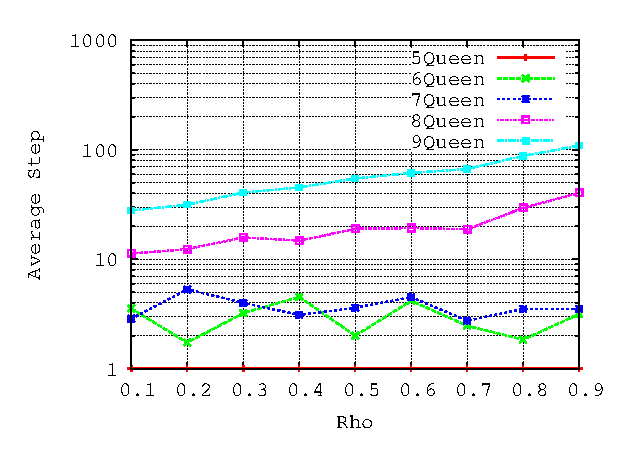
\includegraphics[width=120mm]{image/rho.eps}
	\caption{持続率$\rho$を変化させた結果}
	\label{fig:rho}
\end{center}
\end{figure}

\subsection{$\alpha$を変化させたときのステップ数}
フェロモンの重み$\alpha$を変化させてステップ数の変化をみた結果を図\ref{fig:alpha}に示した.この結果から,解を求めるまでのステップ数が小さい$5,6,7$Queenではフェロモンの重みの影響は大きくないが,ステップ数が大きくなる$8,9$Queenでは,フェロモンの重みが大きくなるほど,ステップ数が小さくなっていることがわかる.
\begin{figure}[H]
\begin{center}
	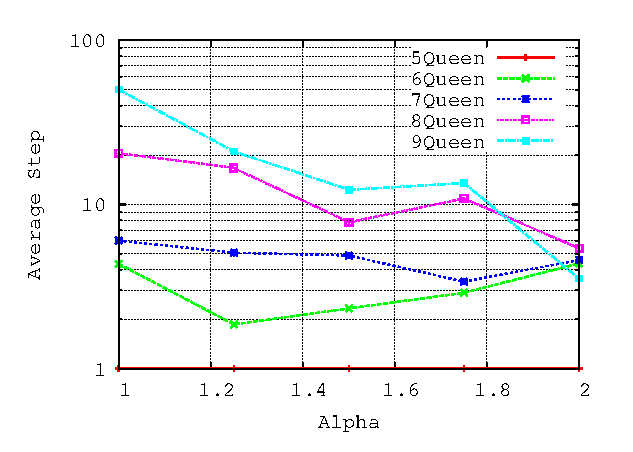
\includegraphics[width=120mm]{image/alpha.eps}
	\caption{フェロモンの重み$\alpha$を変化させた結果}
	\label{fig:alpha}
\end{center}
\end{figure}


\subsection{$\beta$を変化させたときのステップ数}
ヒューリスティックの重み$\beta$を変化させてステップ数の変化をみた結果を図\ref{fig:beta}に示した.この結果から,ヒューリスティックの重みを大きくすると解が求まるまでのステップ数が小さくなっていることがわかる.
\begin{figure}[H]
\begin{center}
	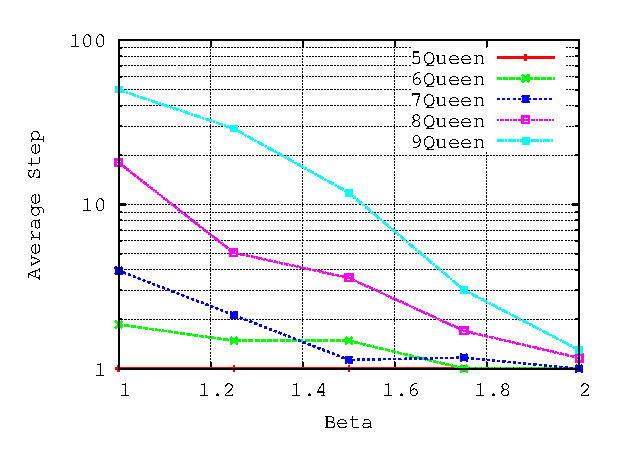
\includegraphics[width=120mm]{image/beta.eps}
	\caption{ヒューリスティックの重み$\beta$を変化させた結果}
	\label{fig:beta}
\end{center}
\end{figure}


\subsection{解の収束率}
持続率$\rho$,フェロモンの重み$\alpha$,ヒューリスティックの重み$\beta$を変化させて解が求まらない回数を見た結果を図\ref{fig:unres_rho},\ref{fig:unres_alpha},\ref{fig:unres_beta}に示した.この結果から,$\rho$と$\beta$を大きくすると解が求まる確率が大きくなり,$\alpha$を大きくすると解が求まる確率が小さくなっていることがわかる.
\begin{figure}[H]
\begin{center}
	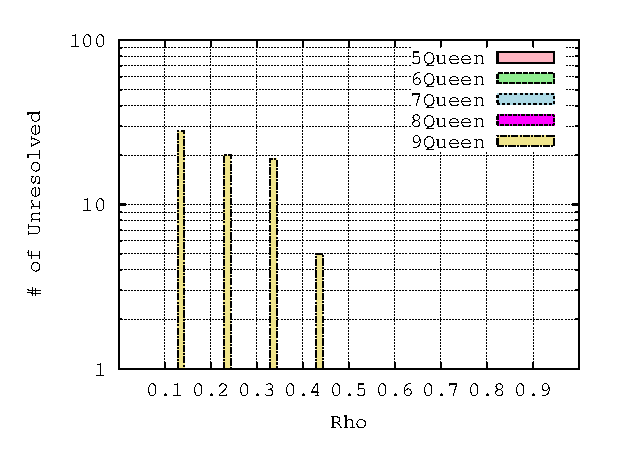
\includegraphics[width=120mm]{image/unresolved_rho.eps}
	\caption{解が求まらなかった回数($\rho$)}
	\label{fig:unres_rho}
\end{center}
\end{figure}
\begin{figure}[H]
\begin{center}
	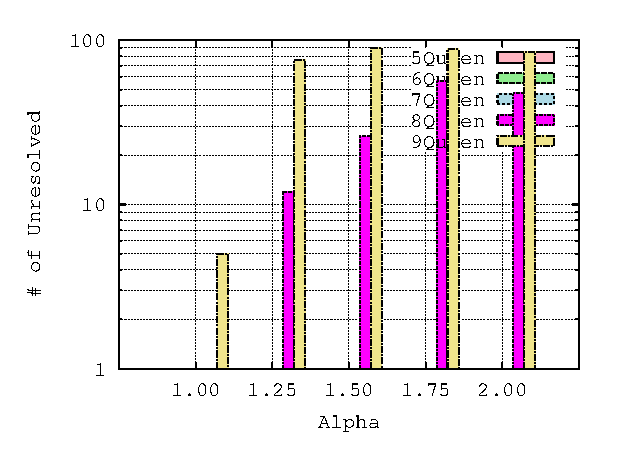
\includegraphics[width=120mm]{image/unresolved_alpha.eps}
	\caption{解が求まらなかった回数($\alpha$)}
	\label{fig:unres_alpha}
\end{center}
\end{figure}
\begin{figure}[H]
\begin{center}
	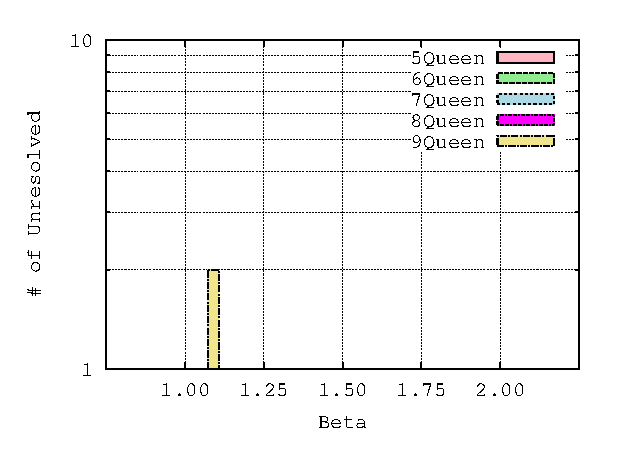
\includegraphics[width=120mm]{image/unresolved_beta.eps}
	\caption{解が求まらなかった回数($\beta$)}
	\label{fig:unres_beta}
\end{center}
\end{figure}




% ---
\section{考察}
\subsection{$\rho$を変化させたときのステップ数}
\label{sec:think_rho}
持続率$\rho$を変化させたときのステップ数の変化が,持続率が大きくなるほどステップ数が大きくなっていることがわかった.したがって,蒸発率を大きくすることでステップ数が減ることがわかった.これは,持続率を上げるほど,全体のフェロモンの値が大きくなり,フェロモンの更新の際に加えた値の影響がなかなか大きくならないためであると考えられる.

これは,前回の課題の焼きなまし法で,温度をゆっくりと下げていく様子に類似している.温度を下げるのがゆっくりであるほど,局所的に良い解に陥ることは少なくなるため,最適解が求まらないということは少なくなるが.試行回数が増えてしまうと推察できる.

また,$N$が小さいときに,ステップ数には大きな影響を与えなかったことは,たまたま解けてしまった場合あるいは時間がかかってしまった場合があり,誤差が大きくなったためと考えられる.


\subsection{$\alpha$を変化させたときのステップ数}
\label{sec:think_alpha}
フェロモンの重み$\alpha$を変化させたときのステップ数の変化は,フェロモンの重みが大きくなるほど小さくなっていくことがわかった.これは,収束する場合に限って,アリのフェロモンを大きくすることで少ないステップで解が求まっただけであり,間違った局所的な最適解に陥ると収束までに時間がかかってしまうと推察される.


\subsection{$\beta$を変化させたときのステップ数}
\label{sec:think_beta}
ヒューリスティックの重み$\beta$を大きくすると,ステップ数が大きく減少することがわかった.これは,アリの移動の際に,ヒューリスティックの値が大きく影響することになるからである.例えば,Queenが死ぬ数が$0$のときと$1$のときでは,ヒューリスティックの値はそれぞれ$1/1=1$,$1/2=0.5$となる.$\beta$の値を大きくすると,前者は$1$のままであるが,後者は$0$に近づいていく.これを移動する確率にかけることになるため,ヒューリスティックの重みが大きい場合,Queenが死ぬ数が$0$のセルに移動する確率はそのままで,死ぬ数が多いセルほど移動する確率が$0$に近づく.

つまり,バックトラックのような処理をアリの数だけ行うことになる.NQueenのような問題では,巡回セールス問題などとは異なり,コスト(NQueenではクイーンが死ぬ数,巡回セールスマン問題では道の長さ)が大きくなる経路は解とはならないため通るべきではない.よって,バックトラックのようになる$\beta$を大きくする,手法がよりステップ数を減らせたといえる.

本課題では,問題のサイズが大きくなると時間が大きくかかるために,複数回の実験を行うことはできなかったが,$\beta$を更に大きくして,実験を数回行った結果,以下のような結果を得た.

\begin{itemize}
	\item $N = 10, rho = 0.300000, alpha = 1.000000, beta = 10.000000$の場合\\
		$100$回試行して平均$1.0$ステップ
	\item $N = 20, rho = 0.300000, alpha = 1.000000, beta = 10.000000$の場合\\
		$10$回試行して平均$1.1$ステップ
	\item $N = 30, rho = 0.300000, alpha = 1.000000, beta = 10.000000$の場合\\
		$5$回試行して平均$2.2$ステップ
	\item $N = 40, rho = 0.300000, alpha = 1.000000, beta = 10.000000$の場合\\
		$1$回試行して$14$ステップ
\end{itemize}

このように,$\beta$が大きければ非常に少ないステップで解にたどり着くことが確かめられた.


\subsection{解の収束率}
持続率$\rho$,フェロモンの重み$\alpha$,ヒューリスティックの重み$\beta$を変化させて解が求まらない回数を見た結果,$\rho$と$\beta$を大きくすると解が求まる確率が大きくなり,$\alpha$を大きくすると解が求まる確率が小さくなってしまうことがわかった.

$\rho$の場合は,\ref{sec:think_rho}節でも述べたように,$\rho$を大きくすることで焼きなまし法でゆっくりと温度を下げていくことと同様の操作となり,ステップ数は増えてしまうが大局的最適解の求まる確率は大きくなるからであると考察できる.

$\alpha$の場合は,\ref{sec:think_alpha}節でも述べたように,$\alpha$を大きくすると,ステップ数の上限までで収束する場合は,たまたま良い解へ向かっていったためであり,実際は大域的最適解に到達できる確率が小さくなってしまうことがわかる.

$\beta$の場合は,\ref{sec:think_beta}節で述べたように,バックトラック法に近い手法を用いるため,最適な解を優先して探すため,大局的最適解にたどり着く確率が非常に大きいと結論できる.


% --
\section{結論}
本課題では,ACOアルゴリズムを用いて,Nクイーン問題の解を求めるプログラムを作成し,このアルゴリズムが確かに正しい解を求めること,パラメータによってその探索ステップが異なることが確かめられた.また,Nクイーン問題に対しては,ACOアルゴリズムよりも,バックトラック法のほうが有効であることが示された.




\begin{thebibliography}{n}
\bibitem{ref:aco}
S. Khan et al.“Solution of n-Queen problem using ACO”. In proc. of 13th IEEE International Multi-topic Conference (INMIC 2009),2009.,\url{http://www.iba.t.u-tokyo.ac.jp/~iba/AI/khan.pdf}


\end{thebibliography}


\appendix
\section{ソースリスト}

ソースのリストを以下に示した.

\begin{itemize}
	\item Makefile \\
		makeをするためのファイル
	\item util.c / util.h \\
		汎用的に用いる関数群.メモリの確保などを含んでいる.
	\item aco.c / aco.h \\
		Nクイーン問題を解く,ACOアルゴリズムを実装したもの.
	\item main.c \\
		ACOアルゴリズムを呼び出すメイン関数.問題の大きさを入力するなどの機能を持つ..
\end{itemize}

\end{document}













